\documentclass[12pt]{extarticle}
\usepackage{graphicx}
\usepackage[utf8]{inputenc}
\usepackage{amsmath}
\usepackage{titlesec}
\usepackage{titling}
\usepackage{xcolor}
% \usepackage{txfonts}  % commented out due to color stack issues
\usepackage{booktabs}
\usepackage{amsfonts}
\usepackage[shortlabels]{enumitem}
\usepackage{latexsym}
\usepackage{fixmath}
\usepackage{hyperref}
\usepackage{amssymb}
\usepackage[italian]{babel}
\usepackage{gensymb}
\usepackage{centernot}
\usepackage{tikz}
\usepackage{mdframed}
\usepackage{listings}
\usepackage[T1]{fontenc}
\usepackage[most]{tcolorbox}
\usepackage{lipsum}
\usepackage{python}
\usepackage[top=2cm, bottom=2cm, left=2cm, right=2cm]{geometry}

\titlespacing*{\section}{0pt}{3.5ex plus 1ex minus .2ex}{2ex plus .2ex}
\titlespacing*{\subsection}{0pt}{3ex plus 1ex minus .2ex}{1.2ex plus .2ex}

\newtcolorbox{cbox}[1]{
    colback=orange!5!white,
    colframe=orange!40!black,
    fonttitle=\bfseries,
    title=#1,
    arc=2mm,
    boxrule=0.5mm,
    left=10pt,
    right=10pt,
    top=10pt,
    bottom=10pt,
    before skip=12pt,
    after skip=12pt,
    breakable
}

\title{Ingegneria del Software}
\author{Mattia Masina\\CdL in Informatica -- Università di Bologna}
\date{Anno Accademico 2026/2027}

\definecolor{codegreen}{rgb}{0,0.5,0}
\definecolor{codegray}{rgb}{0.5,0.5,0.5}
\definecolor{codepurple}{rgb}{0.58,0,0.82}
\definecolor{bluegreen}{rgb}{0,0.6,0.6}
\definecolor{darkorange}{rgb}{1.0, 0.55, 0.0}
\definecolor{lightgray}{rgb}{0.83, 0.83, 0.83}
\definecolor{seashell}{rgb}{1.0, 0.96, 0.93}
\definecolor{lightyellow}{rgb}{1.0, 1.0, 1.0}
\definecolor{ghostwhite}{rgb}{0.97, 0.97, 1.0}
\definecolor{deepcarrotorange}{rgb}{0.91, 0.41, 0.17}
\definecolor{aqua}{rgb}{0.0, 1.0, 1.0}
\definecolor{aquamarine}{rgb}{0.5, 1.0, 0.83}
\definecolor{blue-violet}{rgb}{0.54, 0.17, 0.89}
\definecolor{beaver}{rgb}{0.62, 0.51, 0.44}

\lstdefinestyle{mystyle}{
    backgroundcolor=\color{ghostwhite},
    identifierstyle=\color{black},
    commentstyle=\color{codegreen},
    keywordstyle=\color{blue-violet}\bfseries,
    numberstyle=\tiny\color{bluegreen},
    stringstyle=\color{blue},
    basicstyle=\ttfamily\small,
    breakatwhitespace=false,
    breaklines=true,
    captionpos=b,
    keepspaces=true,
    numbers=left,
    numbersep=5pt,
    showspaces=false,
    showstringspaces=false,
    showtabs=false,
    tabsize=2,
    morekeywords={exp, logspace, print, Exception, try, catch, from, import, while, True, False, },
    emphstyle=\color{blue}\bfseries,
    emph={[2]null},
    emphstyle={[2]\color{deepcarrotorange}\bfseries},
    emph={[3]size, length},
    emphstyle={[3]\color{deepcarrotorange}\bfseries},
    morestring=[b]",
    morestring=[b]',
}

\lstset{style=mystyle}

\begin{document}

\maketitle
\newpage

\tableofcontents
\newpage

\section{Introduzione e Contesto: La Produzione del Software}

\subsection{La Trasformazione Digitale e il Contesto Industriale}
\noindent La trasformazione digitale consiste nel \textbf{far vivere meglio le persone grazie al software}. Oggi ci sono \textbf{oltre 180 milioni di sviluppatori} su GitHub (dato 2025), con una crescita di 36 milioni nell'ultimo anno; l'80\% dei nuovi iscritti adotta GitHub Copilot entro la prima settimana.

\begin{cbox}{Leggi Fondamentali}
\begin{itemize}
    \item \textbf{Legge di Wirth}: ``Il software diventa lento più rapidamente di quanto l'hardware diventi più veloce''. Oggi: il codice si moltiplica più rapidamente della nostra capacità di comprenderlo.
    \item \textbf{Legge di Eagleson}: ``Qualsiasi codice che non hai rivisto negli ultimi sei mesi ti sembrerà estraneo''. Oggi: il codice generato da LLM non rivisto riga per riga ti sembrerà tuo finché non si rompe.
\end{itemize}
\end{cbox}

\noindent \textbf{Il Software come Prodotto Industriale.} Il software è \textbf{sempre il prodotto di un processo di sviluppo} che inizia con un'idea e termina con il ritiro. L'industria mondiale cresce al 5--10\% annuo. Il costo di sviluppo tende a crescere con il \textbf{quadrato delle dimensioni} (legge classica); oggi gli assistenti AI abbassano il costo per riga ma non quello di capire, integrare e mantenere sistemi complessi.

\begin{cbox}{Cifre Chiave (SLOC -- Source Lines of Code)}
\begin{tabular}{lr}
    \toprule
    Prodotto & SLOC \\
    \midrule
    NASA Space Shuttle Flight Control & 1,8M \\
    Linux Kernel 4.2 (2016) & 20,2M \\
    Windows NT 5.0 (1998) & 20M \\
    macOS 10.4 (2005) & 86M \\
    Debian 7.0 (2012) & 419M \\
    Google (monorepo, 2025) & 2 miliardi \\
    \bottomrule
\end{tabular}
\end{cbox}

\noindent Red Hat Linux 7.1 (2000): 30M SLOC, ~8.000 persone-anno (modello COCOMO), costo stimato >1 miliardo \$.

\subsection{Definizioni, Classificazioni e Requisiti}
\begin{cbox}{Cosa è il Software: Quattro Prospettive}
\begin{enumerate}
    \item \textbf{Prodotto invisibile, intangibile, duplicabile}, costoso: opera dell'ingegno protetta da copyright.
    \item \textbf{Servizio digitale}: ha un'interfaccia (API), basa su infrastruttura hw/sw/virtuale, garantisce QoS via contratto.
    \item \textbf{Componente di sistema}: può essere \textit{off-the-shelf} (larga diffusione) o \textit{custom} (commissionato).
    \item \textbf{Macchina astratta}: trasforma il computer realizzando funzioni utili; ha un'architettura (struttura + comportamento).
\end{enumerate}
\end{cbox}

\noindent \textbf{Categorie di Software (2025):}
\begin{itemize}
    \item \textbf{Apps ed Ecosistemi Software} (App Store, Play Store, AWS Marketplace)
    \item \textbf{Software as a Service (SaaS)} -- es. Google, Chrome
    \item \textbf{Embedded Software / IoT} -- ``nascosto'' negli oggetti
    \item \textbf{Social Software (Web 2.0)} -- Facebook, X, LinkedIn, wiki, forum
    \item \textbf{Software Libero (Open Source)} -- 4 libertà FSF (uso, studio, distribuzione, miglioramento)
    \item \textbf{API Economy} -- Amazon, Philips Hue, Google Maps, LLM APIs (OpenAI, Anthropic)
    \item \textbf{Agenti e Orchestratori AI} -- entità autonome + coordinatori di flussi multi-agente
\end{itemize}

\begin{cbox}{Classificazione per Tipo di Prodotto: Tre Categorie}
\begin{itemize}
    \item \textbf{Prodotti Generici (OTS -- Off The Shelf)}: creati da un produttore, venduti a molti clienti (es. videogiochi, Office).
    \item \textbf{Sistemi Commissionati (Custom)}: sviluppati per un cliente specifico (es. portale universitario).
    \item \textbf{Servizi in Perpetuo Sviluppo}: sistemi 24/7 in continuo cambiamento (es. Facebook, Amazon, chatbot).
\end{itemize}
\end{cbox}

\begin{cbox}{Distinzione Fondamentale: Requisiti vs Feature}
\begin{itemize}
    \item \textbf{Requisito}: funzione o qualità \textit{testabile} che l'implementazione deve possedere. \textit{Importante per il cliente}.
    \item \textbf{Feature}: insieme di funzioni che permettono l'uso del prodotto in un servizio. \textit{Importante per il fornitore}.
\end{itemize}
\noindent \textit{Esempio e-commerce}: Requisiti = registrazione, carrello, indirizzi, pagamento. Feature = ``Carrello per negozio elettronico'' (es. OpenCart).
\end{cbox}

\subsection{Dipendenze ed Ecosistemi Software}
\noindent \textbf{Grafo delle Dipendenze.} Ogni prodotto software dipende da altri prodotti, che a loro volta dipendono da altri. Si associa a ciascun sistema un \textbf{grafo di dipendenze} i cui nodi sono \textbf{pacchetti software (librerie) in versioni specifiche}. La gestione delle dipendenze è centrale per sicurezza, riproducibilità e manutenibilità.

\medskip
\noindent \textbf{Ecosistemi Software.} Mercati dove si vendono prodotti (App Store) o componenti/servizi (AWS). Caratteristica: collezione di prodotti su piattaforma definita da un'azienda, che si sviluppano ed evolvono nello stesso ambiente.
\begin{itemize}
    \item App Store 2025: 117 miliardi \$ ricavi vs 49 miliardi \$ Google Play; ~142 miliardi download; app AI driver di ricavi importante.
    \item Concentrazione: 20 ``grandi'' sviluppatori incassano ~50\% degli utili.
\end{itemize}

\subsection{Aspetti Legali, Economici e Garanzie}
\begin{cbox}{Copyright e Licenze}
\begin{itemize}
    \item Il software è \textbf{opera dell'ingegno} protetta da copyright (non brevettabile in Europa).
    \item Copia abusiva = reato penale in Italia (L. 248/2000: 6 mesi -- 3 anni carcere).
    \item \textbf{Licenze}: Proprietaria / Public Domain / Open Source (GPL, MIT, Apache, BSD...).
    \item \textbf{Dibattito 2025}: di chi è il codice generato da LLM (Copilot, Claude)? I modelli ``open-weight'' (es. Llama) sono davvero open source?
\end{itemize}
\end{cbox}

\noindent \textbf{SIAE e Decompilazione.} SIAE: registro pubblico per software originali/creativi; deposito su supporto non riscrivibile. \textbf{Decompilazione}: generalmente vietata dalle licenze proprietarie; eccezioni limitate per interoperabilità (direttiva UE 2009/24).

\begin{cbox}{Garanzie: La Regola Pratica}
\noindent Il software commerciale viene venduto \textbf{``as is'' (così com'è), senza garanzie}. Il contratto (EULA) esclude garanzie di commerciabilità, idoneità, assenza virus, accuratezza. Tutto il rischio è sull'utente.
\medskip
\noindent \textbf{Termini tecnici}:
\begin{itemize}
    \item \textbf{Verifica}: aderenza alla specifica (``abbiamo costruito il prodotto giusto?'').
    \item \textbf{Validazione}: accettazione dal cliente (``abbiamo costruito il prodotto che serve?'').
    \item \textbf{Certificazione}: aderenza a specifiche di legge/standard.
\end{itemize}
\end{cbox}

\subsection{Rischi e Qualità del Software}
\noindent \textbf{Rischi del Software:}
\begin{enumerate}
    \item Rischi di sviluppo
    \item Difetti nel software operativo
    \item Rischi di esercizio
    \item \textbf{Allucinazioni durante generazione AI} (nuovo, 2025+)
\end{enumerate}

\begin{cbox}{Casi Studio Recenti}
\begin{itemize}
    \item \textbf{CrowdStrike, 19 luglio 2024}: aggiornamento difettoso Falcon Sensor $\to$ 8,5 milioni di sistemi Windows bloccati, $\ge$10 miliardi \$ danni globali. Settori: aerei, banche, ospedali, emergenze, governi.
    \item \textbf{NATS UK, 15 settembre 2026}: difetto nel National Airspace System $\to$ ~3.000 voli bloccati, 9 aeroporti, 150.000 passeggeri. Terzo guasto rilevante in 3 anni (non attacco informatico).
\end{itemize}
\end{cbox}

\noindent \textbf{Qualità e Difettosità (Difetti/KLoC):}
\begin{center}
\begin{tabular}{lr}
    \toprule
    Contesto & Difetti/KLoC \\
    \midrule
    Peggiori sistemi militari & 55 \\
    Migliori sistemi militari & 5 \\
    Sviluppo Agile (XP) & 1,4 \\
    Apache Web Server (open source) & 0,5 \\
    NASA Space Shuttle & 0,1 \\
    \bottomrule
\end{tabular}
\end{center}

\begin{cbox}{Codice Generato da AI: Allarme Sicurezza (Dati 2025)}
\begin{itemize}
    \item \textbf{Veracode 2025} (100+ LLM testati): \textbf{45\%} del codice generato contiene vulnerabilità.
    \item \textbf{CodeRabbit (dic. 2025)}: codice AI ha probabilità 1,9--2,7$\times$ maggiore di introdurre password deboli, XSS, deserializzazione insicura; \textbf{2,74$\times$} più vulnerabilità del codice umano.
    \item \textbf{Apiiro (giu. 2025)}: $>$10.000 nuove segnalazioni sicurezza/mese in codice AI-generato, 10$\times$ vs dic. 2024.
\end{itemize}
\end{cbox}

\subsection{Evoluzione dell'AI e Visione della Disciplina}
\noindent \textbf{Timeline Gartner:}
\begin{itemize}
    \item 2022: Foundation Models
    \item 2023: Generative AI
    \item 2024: AI Engineering
    \item 2025: Agentic AI
    \item 2026: Orchestratori
\end{itemize}

\begin{cbox}{Avvertimento Gartner}
\noindent Rischio di \textbf{``agent-washing''}; si prevede che \textbf{>40\% dei progetti agentici verrà abbandonato entro il 2027} per mancanza di valore dimostrato. Il 2026 sarà anche anno di disillusione e consolidamento.
\end{cbox}

\noindent \textbf{Studio METR 2025 (RCT: 16 sviluppatori esperti, 246 task reali):}
\begin{itemize}
    \item Con strumenti AI (Cursor + Claude): sviluppatori \textbf{19\% più lenti}, non più veloci.
    \item Previsione pre-task: +24\% velocità; percezione post-task: +20\% velocità. \textit{Percezione $\neq$ realtà misurata}.
    \item Calo maggiore su codice grande e ben noto -- proprio dove l'AI dovrebbe aiutare di più.
\end{itemize}

\noindent \textbf{Impatto su Stack Overflow.} Dal lancio di ChatGPT (nov. 2022), il volume mensile di domande su Stack Overflow è \textbf{crollato}: caso di scuola su come i LLM abbiano cambiato il modo di cercare aiuto nello sviluppo.

\begin{cbox}{Visione dell'Ingegneria del Software: Principi Guida}
\begin{itemize}
    \item \textbf{Software = infrastruttura cruciale} per ogni attività umana/tecnologica; complessità inimmaginabile.
    \item \textbf{Innovazione continua}: adattarsi e imparare costantemente $\to$ competenza chiave.
    \item \textbf{Agile \& DevOps}: processi collaborativi decisivi per dominare la complessità.
    \item \textbf{Responsabilità etica}: il software non è neutrale; considerare impatto sociale.
    \item \textbf{Ingegneria AI-augmented}: agenti conversazionali affiancano lo sviluppatore in scrittura, test, revisione. \textbf{Cambia il modo di lavorare, non l'esigenza di verifica, responsabilità e comprensione profonda}.
\end{itemize}
\end{cbox}

\noindent \textbf{Aspetti Sociali:}
\begin{itemize}
    \item Sviluppo = lavoro di collaborazione in team interdisciplinari; comunicazione, empatia, prospettive diverse sono cruciali.
    \item Software costruito \textit{per le persone}: UX, feedback continuo, diversità/inclusione $\to$ soluzioni più innovative e inclusive.
    \item Il software \textbf{non è solo codice}: è una costruzione sociale che influenza e viene influenzata da chi lo sviluppa e lo usa.
\end{itemize}

\subsection{Risorse Utili}
\begin{itemize}
    \item \url{stackoverflow.com} (volume domande crollato post-ChatGPT)
    \item \url{www.freelancer.com}
    \item \url{best-practice-software-engineering.blogspot.com}
    \item Gruppi LinkedIn per software developers
    \item \url{catless.ncl.ac.uk/Risks/} (database rischi software)
    \item \url{informationisbeautiful.net/visualizations/million-lines-of-code/}
\end{itemize}

\newpage

\section{Essence}

\subsection{Origini della Disciplina e Iniziativa SEMAT}
\noindent Rispetto all'informatica pura, che vanta basi teoriche e matematiche solide e consolidate fin dai lavori di Turing e dalla teoria degli algoritmi, l'\textbf{ingegneria del software è una disciplina giovanissima}. Nata in modo strutturato solo tra la fine degli anni '60 e gli anni '70 (prima ci si limitava a scrivere codice senza porsi problemi metodologici), l'ingegneria del software ha sempre sofferto della mancanza di presupposti teorici comuni e condivisi.

Questa assenza di fondamenta unificate ha provocato una proliferazione incontrollata di approcci: statistiche industriali contano \textbf{oltre un migliaio di metodologie e ricette differenti}. Spesso si tratta di variazioni minime dello stesso concetto sviluppate da singole persone o aziende, che utilizzano vocaboli diversi per descrivere le medesime pratiche o vocaboli identici per descrivere procedure sottilmente disallineate.

\begin{cbox}{I Quattro Sintomi Critici della Frammentazione}
\begin{itemize}
    \item \textbf{Babele terminologica e attriti nel turnover}: quando persone con formazioni diverse entrano nello stesso team, o quando un membro se ne va a metà progetto e viene sostituito, si sprecano intere settimane solo per far capire al nuovo arrivato a che punto si trovi il lavoro e di cosa si stia parlando.
    \item \textbf{Cultura dei documenti vs cultura dei risultati}: per difendersi dalla complessità e dai costi crescenti, le organizzazioni (specie le grandi realtà come Google o Microsoft rispetto alle piccole software house da 6--7 persone) hanno sviluppato una pesante burocrazia documentale. Tuttavia, documentare meticolosamente ogni passo è statisticamente l'attività meno gradita agli sviluppatori, che preferiscono scrivere codice; il risultato è una montagna di documentazione ``write-only'' che finisce presto dimenticata e cestinata.
    \item \textbf{Pratiche non testate sul campo}: la maggior parte di queste ricette metodologiche non è mai stata sottoposta a reale validazione empirica. La loro efficacia resta discutibile e produce esiti disomogenei: anche un professionista esperto in una specifica pratica rischia di fallire quando si sposta in un gruppo che lavora in modo simile ma non identico.
    \item \textbf{Il dilemma dell'insegnamento}: per i docenti è complicato insegnare la materia senza dover ``battezzare'' arbitrariamente un metodo specifico (es. Scrum, XP) a scapito di altri. Essence risolve questo nodo fornendo un quadro di riferimento neutro a monte.
\end{itemize}
\end{cbox}

\medskip
\noindent \textbf{L'Iniziativa SEMAT e la Genesi di Essence.} Per superare lo scontro ideologico tra metodologie contrapposte e dotare la disciplina di solide fondamenta scientifiche, nel 2009 prende vita l'iniziativa internazionale \textbf{SEMAT} (\textit{Software Engineering Method and Theory}).

\begin{cbox}{Tappe Fondamentali di SEMAT}
\begin{itemize}
    \item \textbf{2009 -- Fondazione SEMAT}: promossa da tre figure di spicco dell'informatica accademica e industriale: \textbf{Ivar Jacobson} (co-ideatore di RUP e pioniere dei casi d'uso), \textbf{Bertrand Meyer} (creatore di Eiffel e del paradigma Design by Contract) e \textbf{Richard Soley} (storico presidente di OMG). L'obiettivo primario è definire una teoria rigorosa per l'ingegneria del software.
    \item \textbf{2012 -- Prima Specifica del Kernel}: pubblicazione della prima specifica ufficiale del Kernel di Essence, elaborata attraverso una collaborazione internazionale e validata su casi d'uso concreti.
    \item \textbf{2014 -- Adozione come Standard OMG}: Essence diventa formalmente uno standard dell'\textbf{Object Management Group} (lo stesso consorzio di standardizzazione internazionale di UML e BPMN), sancendone il riconoscimento universale.
\end{itemize}
\end{cbox}

\subsection{Cos'è Essence e i 7 Alpha del Kernel}
\noindent Lungi dall'essere un puro formalismo teorico o un'ennesima sovrastruttura burocratica, Essence è prima di tutto uno \textbf{strumento orientato alla conversazione}, elemento che costituisce il vero filo conduttore dell'intero corso. Serve a consentire a persone con background e ruoli diversi di comunicare efficacemente sullo stato di un progetto software senza fraintendimenti.

\medskip
\noindent \textbf{Metamodello vs Metodo.} Un equivoco comune consiste nel catalogare Essence come un'ulteriore metodologia concorrente (come Scrum o XP). In realtà Essence si colloca a un meta-livello:

\begin{cbox}{I Tre Pilastri Concettuali}
\begin{itemize}
    \item \textbf{Non è un metodo}: non impone un processo prescrittivo rigido, né una sequenza temporale di attività da eseguire alla cieca.
    \item \textbf{È un metamodello}: descrive la struttura invariante e il vocabolario fondazionale comune a qualsiasi metodo di sviluppo software.
    \item \textbf{È universale e agnostico}: è applicabile trasversalmente a paradigmi differenti, integrandosi con Scrum, Kanban, RUP, SAFe o processi interni personalizzati.
\end{itemize}
\end{cbox}

\begin{cbox}{Principio Chiave: Diagnosi vs Cura}
\noindent Il Kernel di Essence svolge una funzione prettamente \textbf{diagnostica, non prescrittiva}:
\begin{itemize}
    \item \textbf{Fornisce la diagnosi}: rileva con precisione lo stato di avanzamento, le incongruenze e i blocchi del progetto (opera come un termometro oggettivo).
    \item \textbf{Non prescrive la cura}: il Kernel non dice al team \textit{come} risolvere il problema emerso o quali attività specifiche implementare.
    \item \textbf{Responsabilità del Team}: decidere quale azione correttiva intraprendere per superare un ostacolo e transitare allo stato successivo rimane una precisa responsabilità del team, che sceglierà le pratiche operative opportune.
\end{itemize}
\end{cbox}

\noindent Essence si compone fondamentalmente di due elementi:
\begin{enumerate}
    \item Un \textbf{Kernel comune}: un insieme essenziale e minimale di concetti universali sempre presenti in ogni sforzo ingegneristico.
    \item Un \textbf{Linguaggio universale}: un formalismo grafico e testuale per formalizzare, comparare, comporre e adattare pratiche ingegneristiche modulari.
\end{enumerate}

\medskip
\noindent \textbf{I 7 Alpha e il Ruolo degli Esiti.} Il Kernel individua 7 elementi cardine, denominati \textbf{Alpha} (\textit{essential things to work with}), che rappresentano gli aspetti vitali da far progredire in qualsiasi iniziativa software.

\begin{cbox}{Cambio di Paradigma}
\noindent La novità sostanziale risiede nella misurazione del progresso: non si valuta più la conformità tramite la mera consegna di documenti formali, bensì il raggiungimento di \textbf{esiti misurabili e oggettivi} (\textit{outcomes}).
Ogni Alpha progredisce attraverso una sequenza definita di \textbf{stati di salute}, ciascuno con precisi criteri di soddisfazione verificabili.
\end{cbox}

\noindent Nel panorama generale di un progetto possono esistere molti più elementi da monitorare, e singole pratiche specialistiche possono introdurre o specializzare ulteriori Alpha (o sotto-Alpha). Tuttavia, i \textbf{7 Alpha del Kernel} rappresentano il minimo comune denominatore invariante: sono quegli aspetti basilari che risultano presenti \textit{sempre e comunque} in qualunque progetto software.

\clearpage

\noindent \textbf{Le Tre Aree di Interesse (Areas of Concern).} Per offrire una visione d'insieme chiara e immediata, i 7 Alpha sono raggruppati in tre macro-aree ortogonali, codificate per colore:

\begin{center}
\small
\begin{tabular}{p{3.2cm}p{3.8cm}p{7.6cm}}
    \toprule
    \textbf{Area di Interesse} & \textbf{Alpha Inclusi} & \textbf{Finalità e Focus} \\
    \midrule
    \textbf{Customer} \newline \textit{(Il Cliente)} & \textbf{Opportunità} \newline \textbf{Stakeholder} & Rappresenta il valore per utenti e committenti. Assicura che l'iniziativa risponda a reali bisogni di mercato o di business e generi un impatto effettivo.
    \\ \addlinespace
    \textbf{Solution} \newline \textit{(La Soluzione)} & \textbf{Requisiti} \newline \textbf{Sistema Software} & Riguarda la progettazione e la realizzazione tecnica. Garantisce che la specifica sia coerente e che il software evolva sotto controllo architetturale.
    \\ \addlinespace
    \textbf{Endeavor} \newline \textit{(L'Iniziativa)} & \textbf{Lavoro} \newline \textbf{Team} \newline \textbf{Modo di Lavorare} & Governa le persone, l'organizzazione e le attività. Assicura che le modalità di collaborazione e i flussi operativi siano sostenibili ed efficaci.
    \\
    \bottomrule
\end{tabular}
\end{center}

\medskip
\noindent \textbf{Descrizione dei 7 Alpha:}
\begin{enumerate}
    \item \textbf{Opportunità (\textit{Opportunity})}: il valore di business e le circostanze di mercato o strategiche che giustificano l'investimento e lo sviluppo del prodotto.
    \item \textbf{Stakeholder}: le persone, i gruppi o le organizzazioni interessati all'esito del sistema, i cui requisiti e feedback determinano il successo del progetto.
    \item \textbf{Requisiti (\textit{Requirements})}: cosa il sistema software deve fare e quali vincoli/qualità deve rispettare.
    \item \textbf{Sistema Software (\textit{Software System})}: il manufatto tangibile in costruzione, comprensivo di codice, test, configurazioni e documentazione operativa.
    \item \textbf{Lavoro (\textit{Work})}: la suddivisione delle attività, i task e l'impegno operativo necessario per raggiungere gli obiettivi prefissati.
    \item \textbf{Team}: il gruppo di persone che collabora attivamente alla realizzazione delle attività di progetto.
    \item \textbf{Modo di Lavorare (\textit{Way of Working})}: l'insieme delle pratiche, convenzioni, accordi interni e strumenti adottati dal team per cooperare.
\end{enumerate}

\begin{figure}[htbp]
     \centering
      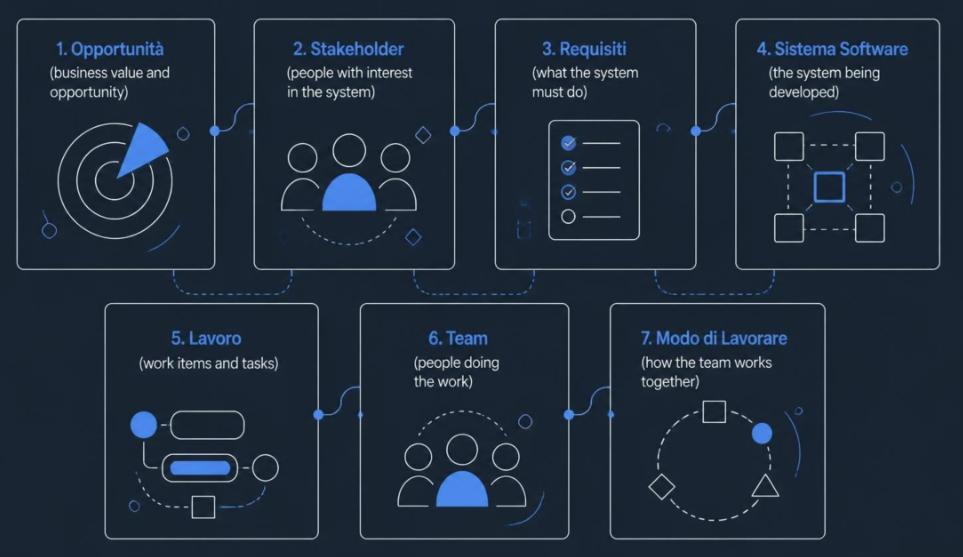
\includegraphics[width=0.88\textwidth]{7alpha.png}
     \caption{I 7 Alpha del Kernel di Essence e la suddivisione nelle tre Aree di Interesse.}
     \label{fig:essence_7_alpha}
\end{figure}

\subsection{Strumenti Pratici, Metodologie e Formazione}
\noindent Una peculiarità di Essence è la traduzione del Kernel in un formato fisico: \textbf{mazzi di carte da gioco}.
Questo consente sia una consultazione rapida da parte dei singoli professionisti, sia la facilitazione di dinamiche partecipative strutturate all'interno del team.

\begin{cbox}{Tecniche e Serious Games}
\begin{itemize}
    \item \textbf{Progress Poker}: ciascun membro valuta indipendentemente lo stato corrente di un Alpha giocando la carta corrispondente; le discrepanze emerse stimolano il confronto per giungere a una stima condivisa e oggettiva.
    \item \textbf{Milestone Mapping}: il team stabilisce le milestone progettuali definendo con precisione quali stati di quali Alpha devono essere soddisfatti per il traguardo, ottenendo una roadmap priva di ambiguità.
    \item \textbf{Checkpoint}: sessioni periodiche di audit per esaminare lo stato di salute generale del sistema attraverso le checklist degli stati degli Alpha.
\end{itemize}
\end{cbox}

\medskip
\noindent \textbf{Integrazione con le Metodologie Esistenti.} Essence non intende sostituirsi ai framework agili o prescrittivi esistenti (Scrum, Kanban, SAFe), ma si propone come loro integratore sistemico:

\begin{cbox}{Valore Aggiunto di Essence sulle Metodologie}
\begin{itemize}
    \item \textbf{Integrazione, non sostituzione}: formalizza con un vocabolario neutro ciò che una metodologia prescrive e ne evidenzia i confini (es. Scrum struttura il \textit{Lavoro} e il \textit{Team}, ma non fornisce pratiche per l'architettura del \textit{Sistema Software}).
    \item \textbf{Identificazione delle lacune}: consente di diagnosticare tempestivamente quali Alpha sono trascurati all'interno dell'organizzazione.
    \item \textbf{Pratiche componibili come building blocks}: permette di trattare le pratiche ingegneristiche (es. User Stories, Standup, TDD, Code Review) come componenti modulari combinabili a piacere per definire un processo su misura (\textit{tailored}).
\end{itemize}
\end{cbox}

\medskip
\noindent \textbf{Essence nella Formazione Universitaria.} Per uno studente di ingegneria del software, studiare Essence fornisce vantaggi strutturali rispetto all'apprendimento mnemonico di un singolo processo:
\begin{enumerate}
    \item \textbf{Pensiero critico sui processi}: capacità di analizzare qualunque metodologia chiedendosi cosa copra, cosa ometta e se sia adatta allo specifico contesto operativo.
    \item \textbf{Risoluzione strutturata dei problemi}: adozione di una griglia diagnostica formale per localizzare dove e perché un progetto manifesti criticità (es. mancato allineamento degli \textit{Stakeholder} vs inefficienze nel \textit{Modo di Lavorare}).
    \item \textbf{Adattabilità al contesto industriale reale}: preparazione a operare in contesti aziendali eterogenei e a partecipare attivamente all'evoluzione dei processi di sviluppo.
\end{enumerate}

\subsection{Metodi, Pratiche e Ciclo di Vita degli Alpha}
\noindent L'esperienza industriale dimostra come l'adozione acritica di metodologie formalizzate spesso non conduca ai benefici sperati. I fattori determinanti di tale inefficacia includono:
\begin{itemize}
    \item \textbf{Elefantiasi prescrittiva}: i metodi tradizionali tendono ad accumulare nel tempo una sovrabbondanza di ruoli specialistici, artefatti documentali e cerimonie burocratiche che appesantiscono il flusso di lavoro.
    \item \textbf{Adozione nominale (Cargo Cult)}: le organizzazioni adottano sovente la terminologia esteriore di una metodologia (es. chiamare le riunioni \textit{Standup} o i requisiti \textit{User Story}), senza modificare la sostanza delle pratiche operative sottostanti.
    \item \textbf{Discrepanze terminologiche}: metodologie differenti impiegano vocaboli differenti per descrivere le medesime problematiche essenziali, ostacolando il confronto oggettivo e il riuso della conoscenza.
    \item \textbf{Focus sugli artefatti vs focus sugli esiti}: i report di avanzamento convenzionali misurano la quantità di documenti prodotti anziché i risultati concreti (\textit{outcomes}) e il reale stato di salute del progetto.
\end{itemize}

\begin{cbox}{La Risposta di Essence}
\noindent Essence affronta queste criticità introducendo una netta separazione delle preoccupazioni:
\begin{itemize}
    \item \textbf{Linguaggio comune minimale}: stabilisce un terreno condiviso (\textit{common ground}) per tutta l'ingegneria del software.
    \item \textbf{Separazione tra universale e contingente}: isola i concetti invarianti di qualsiasi iniziativa rispetto alle guide operative specifiche delle singole pratiche.
    \item \textbf{Progresso visibile e basato su evidenze}: sostituisce la conformità documentale con stati oggettivi e checkpoint verificabili.
    \item \textbf{Composizione ed evoluzione autonoma}: consente ai singoli team di assemblare e far evolvere il proprio modo di lavorare su misura.
\end{itemize}
\end{cbox}

\medskip
\noindent \textbf{Tassonomia: Processo, Metodo e Pratica.} Per comprendere l'architettura di Essence è indispensabile distinguere nettamente tre concetti spesso confusi in letteratura:

\begin{center}
\small
\begin{tabular}{p{3.2cm}p{11.5cm}}
    \toprule
    \textbf{Concetto} & \textbf{Definizione e Ruolo Operativo} \\
    \midrule
    \textbf{Processo (\textit{Process})} & Descrive un \textbf{flusso ordinato di lavoro nel tempo}, specificando sequenze, transizioni e dipendenze temporali tra attività. \\
    \addlinespace
    \textbf{Metodo (\textit{Method})} & Fornisce a un team una \textbf{guida complessiva e strutturata} per condurre un'iniziativa (\textit{endeavour}) dal principio alla conclusione. \\
    \addlinespace
    \textbf{Pratica (\textit{Practice})} & Approccia e risolve un \textbf{aspetto specifico del lavoro} (es. stima a punti, retrospettive, TDD, code review); è modulare e componibile con altre pratiche. \\
    \bottomrule
\end{tabular}
\end{center}

\begin{cbox}{I Metodi come Composizione di Pratiche}
\noindent In Essence, \textbf{un metodo non è un monolite, ma una composizione modulare di pratiche}. 
\medskip

\noindent Questa visione poggia su tre presupposti cardine:
\begin{enumerate}
    \item L'ingegneria del software possiede un \textbf{terreno comune invariante} (\textit{Kernel}).
    \item I metodi sono assemblati selezionando e coordinando singole pratiche specialistiche.
    \item I team devono concentrarsi sull'\textbf{essenziale} e sulla raccolta di \textbf{evidenze oggettive}.
\end{enumerate}
\medskip
\noindent \textit{Metafora dell'Albero}: Il Kernel rappresenta l'albero (la struttura portante comune e stabile), mentre le pratiche costituiscono le decorazioni e le luci che ogni organizzazione sceglie di appendere per personalizzare il proprio modo di lavorare.
\end{cbox}

\medskip
\noindent \textbf{Anatomia di un Alpha: Cicli di Vita, Stati e Checkpoint.} Un Alpha non è un documento, un deliverable o un modello. È una \textbf{preoccupazione essenziale} (\textit{essential concern}) che possiede:
\begin{itemize}
    \item Un \textbf{ciclo di vita esplicito} articolato attraverso una sequenza ordinata di \textbf{stati di salute}.
    \item Una natura agnostica rispetto alla documentazione: \textbf{più prodotti di lavoro (\textit{Work Products}) differenti} possono concorrere a fornire l'evidenza necessaria per uno stesso Alpha.
    \item Universalità: mantiene il suo significato invariato indipendentemente dal metodo adottato (sia esso Waterfall, Scrum o XP).
\end{itemize}

\noindent Ciascun passo nel ciclo di vita di un Alpha è definito da due costrutti precisi:
\begin{itemize}
    \item \textbf{Stato (\textit{State})}: condizione significativa e verificabile lungo il ciclo di vita dell'Alpha.
    \item \textbf{Checkpoint}: elenco rigoroso delle evidenze tangibili richieste per certificare il raggiungimento dello stato corrispondente.
    \item \textbf{Proprietà cumulativa}: uno stato successivo incorpora intrinsecamente il soddisfacimento di tutti gli stati precedenti (\textit{a later state includes the intent of earlier states}).
\end{itemize}

\begin{figure}[htbp]
     \centering
     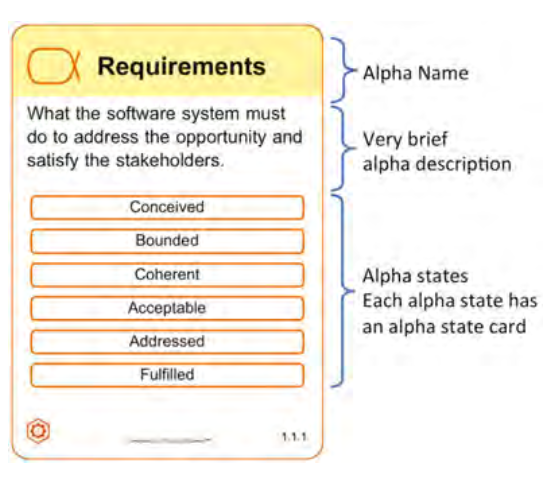
\includegraphics[width=0.45\textwidth]{card.png}
     \caption{Anatomia di una carta Alpha di Essence e gerarchia degli stati con checklist.}
     \label{fig:card}
\end{figure}

\begin{cbox}{I 7 Alpha del Kernel e i Relativi Stati Ordinati}
\begin{enumerate}
    \item \textbf{Customer}:
    \begin{itemize}
        \item \textbf{Opportunity}: \textit{Identified} $\to$ \textit{Solution Needed} $\to$ \textit{Value Established} $\to$ \textit{Viable} $\to$ \textit{Addressed} $\to$ \textit{Benefit Accrued}.
        \item \textbf{Stakeholders}: \textit{Recognized} $\to$ \textit{Represented} $\to$ \textit{Involved} $\to$ \textit{In Agreement} $\to$ \textit{Satisfied for Deployment} $\to$ \textit{Satisfied in Use}.
    \end{itemize}
    \item \textbf{Solution}:
    \begin{itemize}
        \item \textbf{Requirements}: \textit{Conceived} $\to$ \textit{Bounded} $\to$ \textit{Coherent} $\to$ \textit{Acceptable} $\to$ \textit{Addressed} $\to$ \textit{Fulfilled}.
        \item \textbf{Software System}: \textit{Architecture Selected} $\to$ \textit{Demonstrable} $\to$ \textit{Usable} $\to$ \textit{Ready} $\to$ \textit{Operational} $\to$ \textit{Retired}.
    \end{itemize}
    \item \textbf{Endeavour}:
    \begin{itemize}
        \item \textbf{Work}: \textit{Initiated} $\to$ \textit{Prepared} $\to$ \textit{Started} $\to$ \textit{Under Control} $\to$ \textit{Concluded} $\to$ \textit{Closed}.
        \item \textbf{Team}: \textit{Seeded} $\to$ \textit{Formed} $\to$ \textit{Collaborating} $\to$ \textit{Performing} $\to$ \textit{Adjourned}.
        \item \textbf{Way of Working}: \textit{Principles Established} $\to$ \textit{Foundation Established} $\to$ \textit{In Use} $\to$ \textit{In Place} $\to$ \textit{Working Well} $\to$ \textit{Retired}.
    \end{itemize}
\end{enumerate}
\end{cbox}

\noindent \textbf{Relazioni intercorrenti tra gli Alpha.} Gli Alpha non procedono in isolamento, ma interagiscono dinamicamente:
\begin{itemize}
    \item L'\textbf{Opportunity} guida ed orienta la specifica dei \textbf{Requirements}.
    \item Gli \textbf{Stakeholders} utilizzano, valutano e supportano il \textbf{Software System}.
    \item Il \textbf{Team} pianifica, coordina ed esegue il \textbf{Work}.
    \item Il \textbf{Way of Working} disciplina e sostiene contestualmente sia il \textbf{Team} sia il \textbf{Work}.
\end{itemize}

\medskip
\noindent \textbf{Progresso vs Salute del Progetto.} Nell'ingegneria del software, Valore, Soluzione e Iniziativa evolvono congiuntamente ma a velocità spesso disomogenee. Le metriche di avanzamento tradizionali (es. \textit{burndown chart}, ore lavorate, task completati) tendono a mascherare anomalie critiche: un progetto può apparire perfettamente in orario mentre accumula un debito di rischio insostenibile su un Alpha trascurato.

\begin{cbox}{Progresso vs Salute (Health)}
\begin{itemize}
    \item \textbf{Progresso (\textit{Progress})}: misura quantitativa di quanto un singolo Alpha sia avanzato lungo la sua sequenza di stati di salute.
    \item \textbf{Salute (\textit{Health})}: valutazione qualitativa sull'idoneità dello stato attuale dell'Alpha a sostenere l'iniziativa senza compromettere gli altri elementi del Kernel.
    \item \textbf{Ostacoli al prossimo stato (\textit{Next-state obstacles})}: l'attenzione diagnostica del team non deve limitarsi a certificare lo stato raggiunto, ma deve identificare tempestivamente le barriere che impediscono il soddisfacimento dei checkpoint dello stato immediatamente successivo.
\end{itemize}
\end{cbox}

\subsection{Elementi Complementari e Studio di Caso (UniMagic)}
\noindent \textbf{Work Products vs Alpha.} Un \textbf{Work Product} è un artefatto tangibile e contingente (es. il Product Backlog di Jira, un diagramma delle classi, una build eseguibile, una specifica di collaudo).
\begin{itemize}
    \item La produzione di un Work Product \textbf{non implica automaticamente l'avanzamento di stato dell'Alpha}. Ad esempio, scrivere un documento di 200 pagine non fa transitare i \textit{Requirements} allo stato \textit{Coherent} se persistono contraddizioni o se gli stakeholder non hanno validato i casi d'uso critici.
    \item L'artefatto assume valore ingegneristico esclusivamente quando fornisce l'\textbf{evidenza} idonea a soddisfare i checkpoint dell'Alpha corrispondente.
\end{itemize}

\medskip
\noindent \textbf{Attività e Spazi di Attività (Activity Spaces):}
\begin{itemize}
    \item \textbf{Spazio di Attività (\textit{Activity Space})}: definisce un'area di lavoro universale e invariante prevista dal Kernel (il \textit{``cosa fare''} ad alto livello, es. \textit{Explore Possibilities}, \textit{Coordinate Activity}).
    \item \textbf{Attività (\textit{Activity})}: rappresenta l'unità esecutiva di lavoro definita da una specifica pratica adottata (il \textit{``come farlo''}, es. \textit{Sprint Planning}, \textit{Code Review}).
    \item Il mapping tra le attività concrete e gli Activity Spaces del Kernel consente di identificare immediatamente duplicazioni, ridondanze o lacune metodologiche nell'organizzazione.
\end{itemize}

\medskip
\noindent \textbf{Competenze e Pattern:}
\begin{itemize}
    \item \textbf{Competenze (\textit{Competencies})}: abilità, conoscenze ed esperienze formali richieste alle figure umane per condurre specifici compiti ingegneristici.
    \item \textbf{Pattern}: soluzioni standardizzate e riutilizzabili a problemi ricorrenti. In questo metamodello, i \textbf{Ruoli} (es. Scrum Master, Product Owner, Tech Lead) sono formalizzati come pattern composti che aggregano insiemi coerenti di responsabilità e competenze.
\end{itemize}

\begin{figure}[htbp]
     \centering
     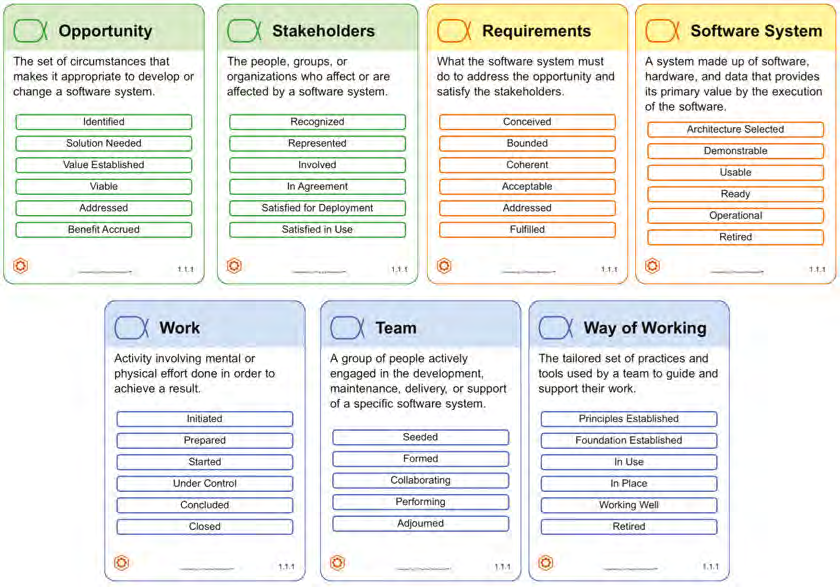
\includegraphics[width=0.9\textwidth]{AlphaCards.png}
     \caption{Anatomia di una carta Alpha di Essence e gerarchia degli stati con checklist.}
     \label{fig:AlphaCards}
\end{figure}

\medskip
\noindent \textbf{Studio di Caso Applicativo: Diagnosi del Progetto UniMagic.} Una software house fondata di recente da circa 12 persone (prevalentemente sviluppatori web) riceve il suo primo incarico commerciale significativo dall'\textit{Università di Warthog}. Il progetto consiste nello sviluppo di \textbf{UniMagic}, una piattaforma digitale per unificare la gestione del supporto ai corsi, la prenotazione degli appuntamenti e le istanze amministrative degli studenti.

\medskip
\noindent \textbf{Vincoli e Condizioni di Partenza}:
\begin{itemize}
    \item Rilascio della prima versione operativa a \textbf{2.000 studenti} entro un semestre accademico.
    \item Divergenze e disaccordo tra gli stakeholder in merito alle priorità funzionali e ai vincoli di privacy.
    \item Team di sviluppo composto da 6 persone, con esperienza in ambienti web ma completamente prive di competenze su Essence.
\end{itemize}

\begin{cbox}{Diagnosi degli Alpha dello Scenario (Senza Prescrizione di Cura)}
\begin{itemize}
    \item \textbf{Requirements $\to$ Stato massimo: \textit{Conceived}}:
    L'ambito generale del servizio è stato delineato, ma la persistenza di conflitti non sanati sulle priorità e sulle policy di riservatezza impedisce di considerare i requisiti circoscritti e condivisi. Non è soddisfatto il checkpoint di confine per lo stato \textit{Bounded}.
    \item \textbf{Team $\to$ Stato effettivo: \textit{Formed}}:
    I 6 membri sono stati identificati e assegnati al progetto, ma operano come somma di individualità. Mancano le evidenze oggettive di cooperazione coesa, fiducia reciproca e allineamento sulla missione richieste per lo stato \textit{Collaborating}.
    \item \textbf{Way of Working $\to$ Stato effettivo: \textit{Principles Established}}:
    Il gruppo ha espresso l'intenzione di adottare uno sviluppo iterativo, ma non ha ancora istanziato né validato sul campo strumenti e pratiche operative concordate. L'approccio non è ancora operativamente \textit{In Use}.
\end{itemize}
\end{cbox}

\noindent \textbf{Analisi delle criticità e delle asserzioni non supportate:}
\begin{itemize}
    \item \textbf{Asserzione a rischio}: l'assunzione che il primo rilascio sia pienamente fattibile per 2.000 utenti entro un solo semestre.
    \item \textbf{Evidenza mancante}: non sussistono evidenze relative all'architettura tecnica del \textit{Software System}, alla capacità produttiva misurata del \textit{Team} e alla convergenza contrattuale degli \textit{Stakeholders}. Il progetto presenta un elevato rischio di fallimento latente non rilevabile dai soli diagrammi di pianificazione.
    \item \textbf{Ruolo del Team nella Soluzione}: Essence ha diagnosticato il disallineamento; spetta ora al team definire la strategia risolutiva (es. rinegoziare lo scope con il cliente, introdurre pratiche di prototipazione rapida o adottare spike architetturali).
\end{itemize}

\end{document}